%%%%%%%%%%%%%%%%%%%%%%%%%%%%%%%%%%%%%%%%%%%%%%%%%%%%%%%%%%%%%%%%%%%%%%
% How to use writeLaTeX: 
%
% You edit the source code here on the left, and the preview on the
% right shows you the result within a few seconds.
%
% Bookmark this page and share the URL with your co-authors. They can
% edit at the same time!
%
% You can upload figures, bibliographies, custom classes and
% styles using the files menu.
%
%%%%%%%%%%%%%%%%%%%%%%%%%%%%%%%%%%%%%%%%%%%%%%%%%%%%%%%%%%%%%%%%%%%%%%

\documentclass[12pt]{article}

\usepackage{sbc-template}
\usepackage{amsfonts}
\usepackage{graphicx,url}
\usepackage{float}
%\usepackage[brazil]{babel}   
\usepackage[utf8]{inputenc}
\usepackage{algorithm}
\usepackage[noend]{algpseudocode}

\usepackage{listings}

\usepackage{amsmath}
\usepackage[table]{xcolor}
\usepackage{float}
\usepackage{adjustbox}

\sloppy

\title{Trabalho Prático 1: Busca em Mapas}

\author{Bernardo de Almeida Abreu\inst{1}}


\address{Departamento de Ciência da Computação -- Universidade Federal de Minas Gerais
	\\Disciplina: DCC028 - Inteligência Artificial 2018/1
  \email{bernardoabreu@dcc.ufmg.br}
}

\begin{document} 

\lstset{
    columns=fullflexible,
    keepspaces=true,
    literate={-}{-}1,
    framexleftmargin=2.5mm,
	breaklines=true,
    keepspaces=true,
    prebreak=\textbackslash
}

\maketitle


\section{Introdução}
Esse trabalho possui como objetivo analisar diferentes algoritmos de busca em espaços de estados. Os algoritmos analisados são a busca de aprofundamento iterativa (IDS), busca de custo uniforme (UCS), busca gulosa de melhor escolha (\textit{Best First Search}) e busca A*.

Os mapas nos quais os algoritmos de busca serão executados são bidimensionais, representados por matrizes de caracteres. As células marcadas com um "." estão livres e células marcadas com um "@" estão bloqueadas.


\section{Implementação}
Os algoritmos de busca foram implementados utilizando a linguagem \textit{Python 3}.
Foi criada uma classe \textit{GraphSearch} para implementar o algoritmo de busca em grafo básico, apresentado por~\cite{russell2010artificial}. Cada algoritmo a ser implementado no trabalho, herda da classe \textit{GraphSearch} e implementa as funções necessárias para executar o algoritmo de busca.

% \begin{algorithm}
% \caption{Função de busca em grafo}\label{alg:graph_search}
% \begin{algorithmic}[1]
% \Function{GRAPH\_SEARCH}{$problem$}
%   \State $node \gets problem.$INITIAL\_STATE
%   \State $frontier \gets$ \Call{INIT\_FRONTIER}{{}}\label{call:init_frontier}
%   \State $frontier \gets$ \Call{INSERT}{$frontier, node$}

%   \State $explored\gets \emptyset$
%   \Loop
%     \If {\Call{EMPTY?}{$frontier$}}
%         \State \textbf{return} FAILURE
%     \EndIf

%     \State $frontier, node \gets$ \Call{REMOVE}{$frontier$}

%     \If {\Call{GOAL?}{$problem, node$}}
%         \State \textbf{return} \Call{SOLUTION}{$node$}
%     \EndIf

%     \State $explored \gets explored \cup \{node\}$

%     \ForAll{$action \in $ \Call{GET\_ACTIONS}{$problem,node$}}
%         \State $child \gets $ \Call{CHILD\_NODE}{$problem, node, action$}
%         \State $frontier \gets $ \Call{UPDATE\_FRONTIER}{$child, frontier, explored$}
%     \EndFor
%   \EndLoop\label{searchloop}
% \EndFunction
% \end{algorithmic}
% \end{algorithm}

% A função \textit{GRAPH\_SEARCH} implementa o comportamento básico de todas os algoritmos de busca. As particularidades da implementação de cada algoritmo se referem ao modo como a fronteira será gerenciada em cada algoritmo. Algumas das funções chamadas nesse algoritmo são as seguintes:

% \begin{description}
% \item[INIT\_FRONTIER] Inicializa a fronteira com a estrutura apropriada para o algoritmo a ser utilizado.
% \item[GOAL?] Verifica se o nó corresponde ao objetivo.
% \item[GET\_ACTIONS] Retorna uma lista de ações válidas para o nó.
% \item[CHILD\_NODE] Cria um novo nó a partir de uma ação.
% \item[UPDATE\_FRONTIER] Atualiza a fronteira de acordo com o tratamento necessário para o algoritmo.
% \end{description}

\subsection{Estruturas}
\subsubsection{Conjunto de estados explorados}
O algoritmo de busca em grafos precisa manter um conjuntos de nós já visitados para que os mesmos não sejam repetidos. Esse conjunto é o conjunto \textit{explorado}. Uma vez que cada estado do problema é representado por uma posição no mapa, ou seja, um par de coordenadas (X,Y), é possível criar uma tabela \textit{hash} com acesso O(1) para guardar quais estados já foram visitados. Essa tabela é implementada por meio de uma matriz booleana, onde \textit{true} indica que o estado já foi visitado e \textit{false} o contrário.

% \subsubsection{Classe \textit{Problem}}
% Foi implementada uma classe \textit{Problem} para representar o problema. Essa classe guarda as informações sobre o estado inicial, o estado objetivo e o mapa onde a busca ocorre. Além disso, ela possui funções para retornar as ações válidas a partir de um estado, para gerar um novo estado a partir de uma ação e para testar se um estado é a solução.

% \subsubsection{Classe \textit{Node}}
% Um nó de busca também é implementado através de uma classe. Essa classe guarda informações sobre o estado do nó, o nó que gerou esse estado, o custo total do caminho encontrado até o momento e a ação que levou a esse estado. A partir dessa classe é possível reconstruir o caminho encontrado para a solução.

\subsubsection{Fronteira}
Foram criadas duas classes para a fronteira. A primeira classe, \textit{Frontier}, implementa a fronteira utilizando uma pilha ou uma lista, selecionável por meio de um parâmetro. Existem funções para inserir e retirar elementos da fronteira, verificar se a mesma está vazia e verificar se um certo elemento se encontra nela. Além disso, existe uma função para substituir um nó presente na fronteira por um nó com o mesmo estado, caso o novo possua um custo de caminho menor. Para verificar se um elemento já se encontra na fronteira, foi utilizada a classe \textit{ExploredSet}, de forma que uma matriz booleana é usada para verificar a presença de um elemento em O(1).

A segunda classe é a \textit{PriorityFrontier}. Ela reimplementa as funções de inserir, remover e substituir para utilizar uma fila de prioridades. As funções de inserir e substituir recebem uma tupla de (prioridade, nó) nessa classe.

\subsection{Busca de aprofundamento iterativa - IDS}
O algoritmo IDS consiste em chamar o método de busca DLS(\textit{Depth Limited Search}) diversas vezes, aumentado iterativamente o limite de profundidade para a nova execução, até que uma solução é encontrada ou o grafo inteiro é percorrido. A profundidade considerada para esse algoritmo foi o custo do caminho, e não a aresta do grafo. Dessa forma o limite é aumentado com um passo de 0.5, e não de 1.

O algoritmo de DLS implementado consiste numa adaptação do algoritmo de busca em grafos apresentado por~\cite{russell2010artificial}. A estrutura de fronteira utilizada no algoritmo é uma pilha, implementada por meio da classe \textit{Frontier}. Além disso, o método de atualização da fronteira, mostrado pelo algoritmo~\ref{alg:update_frontier_ids}, é um pouco diferente. Caso o custo do caminho para o nó que acabou de ser gerado seja maior do que o limite, é indicado que o limite foi atingido e mais nada é feito. Caso o estado do nó não esteja presente na fronteira, ou no conjunto de explorados, o mesmo é adicionado a fronteira.

A terceira condição da função \textit{UPDATE\_FRONTIER}, indicada na linha~\ref{ids:cost}, existe pois esse algoritmo consiste em uma busca em profundidade com um conjunto de nós visitados. Dessa forma, um nó pode ser visitado primeiro por um caminho mais longo, e depois por um caminho mais curto, o que deve ser levado em consideração pelo algoritmo para se obter o caminho correto. Portanto, o conjunto de explorados utilizado nesse algoritmo é um pouco diferente do tradicional. A classe \textit{ExploredCosts} foi criada, herdando de de \textit{ExploredSet}, de forma a guardar o custo dos caminhos explorados, ao invés de um valor booleano. Assim, a terceira condição verifica se o nó gerado já foi explorado com um caminho maior do que o atual, para que se possa repetir a busca caso o novo caminho seja melhor.


\begin{algorithm}
\caption{Atualiza a fronteira do IDS}\label{alg:update_frontier_ids}
\begin{algorithmic}[1]
\Function{UPDATE\_FRONTIER}{$child, frontier, explored, limit$}
	\If {$child.$PATH\_COST $> limit$}
    	\State $limit\_reached \gets true$
	\ElsIf{$child.$STATE $\notin frontier$ \textbf{and} $child.$STATE $ \notin explored$}
    	\State $frontier \gets$ \Call{INSERT}{$frontier, child$}
    \ElsIf {\Call{GET\_COST}{$explored, child.$STATE} $> child.$PATH\_COST}\label{ids:cost}
    	\State $frontier \gets$ \Call{INSERT}{$frontier, child$}
    \EndIf
\EndFunction
\end{algorithmic}
\end{algorithm}


\subsection{Busca de custo uniforme - UCS}
A fronteira utilizada no algoritmo UCS é uma fila de prioridades, cuja valor de prioridade é o valor do custo do caminho até o nó. A fronteira é atualizada em dois casos distintos. No primeiro caso, caso o estado do nó gerado já esteja presente na fronteira com um custo de caminho maior do que o novo, o mais recente substitui o nó na fronteira. O segundo caso ocorre quando o novo nó não se encontra na fronteira ou no conjunto de explorados, resultando na sua inserção na fronteira.

% \begin{algorithm}
% \caption{Atualiza a fronteira do UCS}\label{alg:update_frontier_ucs}
% \begin{algorithmic}[1]
% \Function{UPDATE\_FRONTIER}{$child, frontier, explored$}
%     \If {$child.$STATE $\in frontier$}
%         \State $frontier \gets$ \Call{REPLACE}{$frontier,(child.$PATH\_COST$, child)$}
%     \ElsIf{$child.$STATE $ \notin explored$}
%     	\State $frontier \gets$ \Call{INSERT}{$frontier, (child.$PATH\_COST$, child)$}
%     \EndIf
% \EndFunction
% \end{algorithmic}
% \end{algorithm}


\subsection{Algoritmos de busca com informação}
Para os algoritmos de busca com informação, a busca gulosa e A*, foi implementada uma classe \textit{HeuristicSearch} que herda de \textit{GraphSearch}. Essa classe adiciona a possibilidade de se escolher uma heurística e define a fronteira como uma fila de prioridades.

\subsubsection{Busca gulosa de melhor escolha - \textit{Best first Search}}
O algoritmo de busca gulosa utiliza uma fila de prioridades como sua fronteira, na qual o valor da heurística é utilizado como valor de prioridade. A atualização da fronteira é feita de forma que um novo nó é inserido na fronteira caso já não se encontre na mesma ou no conjunto de estados explorados.

\subsubsection{A*}
O valor de prioridade utilizado no algoritmo A* é o valor da heurística, chamado de $h$, somado com o custo do caminho para o nó, chamado de $g$, de forma que $f = h + g$. A atualização da fronteira segue os mesmos casos do algoritmo UCS. Um nó gerado substitui o nó na fronteira caso o segundo possua um valor de $f$ maior do que o primeiro, e um nó gerado é inserido na fronteira caso não se encontre na mesma ou no conjunto de nós explorados.

\subsubsection{Heurísticas}
Duas heurísticas possíveis foram implementadas, a \textit{distância Manhattan}~(\ref{eq:manhattan}) e a \textit{distância octile}~(\ref{eq:octile}). Entre essas heurísticas, a única admissível e consistente é a \textit{distância octile}.

\begin{equation}\label{eq:manhattan}
\begin{matrix}
dx = abs(node.x - goal.x)\\
dy = abs(node.y - goal.y)\\
h(n) = (dx + dy)\\
\end{matrix}
\end{equation}

\begin{equation}\label{eq:octile}
\begin{matrix}
dx = abs(node.x - goal.x)\\
dy = abs(node.y - goal.y)\\
h(n) = max(dx,dy) + 0.5 \times min(dx,dy)
\end{matrix}
\end{equation}

A \textit{distância Manhattan} não é capaz de diferenciar o custo de se movimentar na diagonal dos outros custos, assim, o valor de custo retornado pela heurística para se andar para um quadrado diretamente na diagonal é $2$, enquanto o valor real é $1.5$. Para uma heurística ser admissível, é necessário que seu valor seja menor ou igual ao valor real, o que não acontece nesse caso.

A \textit{distância octile} leva em consideração os custos das diagonais. O número de passos diagonais em um caminho livre é igual a $min(dx,dy)$. O termo ($0.5\times min(dx,dy)$) pode ser reescrito como ($1.5 \times min(dx,dy) - 1 \times min(dx,dy)$), que corresponde ao números de passos na diagonal que se deve dar, multiplicado pelo custo da diagonal, menos o número de passos que não se está dando na direção de $max(dx,dy)$, por se estar usando a diagonal.

Com um caminho livre, o custo dado para se caminha na horizontal ou vertical é igual ao custo ótimo, uma vez que o valor de min(dx,dy) é 0, e o valor de max(dx,dy) é o próprio valor da distância. Ao se caminhar para o quadrado exatamente na diagonal, o custo total será $1.5$, que corresponde à distância ótima.

Uma heurística é consistente se, para um nó \textit{n} e os seus sucessores \textit{n'} gerados por uma ação \textit{a}, o custo estimado de atingir o objetivo a partir de \textit{n} não é maior que o custo de chegar a \textit{n'} somado ao custo estimado de \textit{n'} para o objetivo~\cite{russell2010artificial}. O custo estimado de se atingir um nó com a heurística de \textit{distância octile} corresponde ao custo ótimo possível dentro de um mapa com caminho livre. Logo o custo real não é menor do que o custo estimado.



\section{Experimentos}
Para realizar o experimento foram gerados 100 pontos válidos para cada mapa, e então selecionados os valores que eram válidos nos 3 mapas.

\subsection{Custo total}
Os pontos avaliados são mostrados nas tabela~\ref{tab:total-costs-1},~\ref{tab:total-costs-2} e~\ref{tab:total-costs-3}. É possível observar que o custo dos algoritmos A* com \textit{distância octile}, UCS e IDS são iguais, uma vez que esses algoritmos são ótimos. Já o custo do algoritmo guloso é, na maioria das vezes, maior do que o ótimo. Isso se deve a sua natureza gulosa, que busca encontrar o primeiro resultado possível, sem se preocupar com o resultado ótimo. Em alguns casos, pode haver uma interrupção no meio do caminho, que o algoritmo guloso não leva em conta previamente, resultando em um caminho total de custo maior.

\begin{table}[htbp]
\centering
\caption{Custo total para o mapa 1}
\label{tab:total-costs-1}
\begin{tabular}{ll|lllll}
\multicolumn{2}{c|}{Points}  & \multicolumn{5}{c}{Total Cost} \\ \hline
Initial & Final & A* Octile & A* Manhattan & BG    & UCS   & IDS   \\ \hline
167,173       & 232,224     & 90.5      & 90.5         & 90.5  & 90.5  & 90.5  \\
92,218        & 184,181     & 110.5     & 110.5        & 111.5 & 110.5 & 110.5 \\
95,165        & 74,69       & 120       & 120          & 124   & 120   & 120   \\
138,133       & 26,160      & 140.5     & 140.5        & 150   & 140.5 & 140.5 \\
193,73        & 246,155     & 214       & 214          & 240   & 214   & 214   \\
174,14        & 53,61       & 241.5     & 241.5        & 293.5 & 241.5 & 241.5 \\
33,218        & 26,98       & 254.5     & 259.5        & 379   & 254.5 & 254.5
\end{tabular}
\end{table}

\begin{table}[htbp]
\centering
\caption{Custo total para o mapa 2}
\label{tab:total-costs-2}
\begin{tabular}{ll|lllll}
\multicolumn{2}{c|}{Points} & \multicolumn{5}{c}{Total Cost}\\ \hline
Initial & Final & A* Octile & A* Manhattan & BG    & UCS   & IDS   \\ \hline
167,173       & 232,224     & 93        & 93           & 94    & 93    & 93    \\
92,218        & 184,181     & 115       & 115.5        & 117   & 115   & 115   \\
95,165        & 74,69       & 214       & 214          & 236   & 214   & 214   \\
138,133       & 26,160      & 365       & 365          & 460.5 & 365   & 365   \\
193,73        & 246,155     & 122.5     & 122.5        & 122.5 & 122.5 & 122.5 \\
174,14        & 53,61       & 154.5     & 154.5        & 238   & 154.5 & 154.5 \\
33,218        & 26,98       & 226.5     & 226.5        & 268.5 & 226.5 & 226.5
\end{tabular}
\end{table}

\begin{table}[htbp]
\centering
\caption{Custo total para o mapa 3}
\label{tab:total-costs-3}
\begin{tabular}{ll|lllll}
\multicolumn{2}{c|}{Points} & \multicolumn{5}{c}{Total Cost}      \\ \hline
Initial & Final & A* Octile & A* Manhattan & BG    & UCS   & IDS  \\ \hline
167,173       & 232,224     & 107       & 107          & 110   & 107   & 107   \\
92,218        & 184,181     & 129       & 129          & 142   & 129   & 129   \\
95,165        & 74,69       & 129.5     & 129.5        & 170   & 129.5 & 129.5 \\
138,133       & 26,160      & 125.5     & 126.5        & 142   & 125.5 & 125.5 \\
193,73        & 246,155     & 171.5     & 171.5        & 174.5 & 171.5 & 171.5 \\
174,14        & 53,61       & 144.5     & 144.5        & 155.5 & 144.5 & 144.5 \\
33,218        & 26,98       & 245       & 245          & 318.5 & 245   & 245  
\end{tabular}
\end{table}

Foram selecionados alguns outros pontos para se comparar melhor as heurísticas para o algoritmo A*, de forma a mostrar que a heurística de \textit{distância Manhattan} não é ótima. Esses pontos são mostrados na tabela~\ref{tab:a-total-costs}. A heurística de \textit{distância octile} é admissível e consistente, portanto a sua utilização torna o algoritmo ótimo. Já a heurística da \textit{distância Manhattan} não é admissível e consistente, de forma que o resultado obtido nem sempre é ótimo, como se pode observar.

\begin{table}[htbp]
\caption{Custos totais para cada heurística do A*}
\label{tab:a-total-costs}
\begin{adjustbox}{max width=\textwidth}
\begin{tabular}{llll|llll|llll}
\multicolumn{4}{c}{Map 1} & \multicolumn{4}{c}{Map 2} & \multicolumn{4}{c}{Map 3} \\ \hline
\multicolumn{2}{c}{Points} & \multicolumn{2}{c}{Total Cost} & \multicolumn{2}{c}{Points} & \multicolumn{2}{c}{Total Cost} & \multicolumn{2}{c}{Points} & \multicolumn{2}{c}{Total Cost} \\ \hline
\multicolumn{1}{c}{Initial} & \multicolumn{1}{c}{Final} & \multicolumn{1}{c}{Manhattan} & \multicolumn{1}{c|}{Octile} & \multicolumn{1}{c}{Initial} & \multicolumn{1}{c}{Final} & \multicolumn{1}{c}{Manhattan} & \multicolumn{1}{c|}{Octile} & \multicolumn{1}{c}{Initial} & \multicolumn{1}{c}{Final} & \multicolumn{1}{c}{Manhattan} & \multicolumn{1}{c}{Octile} \\ \hline
58,112 & 205,70 & 198.0 & 184.0 & 92,218 & 184,181 & 115.5 & 115.0 & 97,165 & 47,236 & 99.5 & 96.5 \\
91,170 & 144,41 & 197.0 & 192.0 & 213,79 & 104,12 & 157.0 & 153.0 & 153,229 & 69,195 & 104.5 & 102.5 \\
163,247 & 215,93 & 225.0 & 217.0 & 251,25 & 92,13 & 166.5 & 166.0 & 58,18 & 149,22 & 105.5 & 104.0 \\
45,70 & 241,106 & 262.5 & 253.0 & 236,125 & 65,162 & 269.0 & 267.5 & 107,145 & 38,205 & 124.0 & 115.5 \\
33,218 & 26,98 & 259.5 & 254.5 & 200,249 & 147,16 & 325.5 & 320.5 & 138,133 & 26,160 & 126.5 & 125.5 \\
212,2 & 69,180 & 262.5 & 259.5 & 225,229 & 32,55 & 325.0 & 322.5 & 212,163 & 135,232 & 146.0 & 145.5 \\
189,12 & 113,184 & 267.5 & 264.5 & 249,134 & 34,130 & 372.5 & 371.0 & 85,17 & 164,127 & 151.0 & 150.0 \\
57,238 & 4,11 & 334.5 & 329.5 & 244,213 & 54,68 & 384.0 & 380.5 & 30,93 & 152,2 & 200.5 & 196.5 
\end{tabular}
\end{adjustbox}
\end{table}


\subsection{Estados expandidos}
O número total de nós expandidos para cada algoritmo é mostrado nas figuras~\ref{fig:expanded1},~\ref{fig:expanded2} e~\ref{fig:expanded3}. Como é possível observar, a quantidade de nós expandidos no algoritmo IDS é muito grande. Isso se deve em parte ao fato de o algoritmo executar por diversas iterações, de forma que algumas expansões são repetidas a cada iteração. Nas iterações em que o limite de profundidade não permite que uma solução seja encontrada, serão expandidos todos os estados dentro do limite.

\begin{figure}[!htb]
\begin{minipage}{0.5\linewidth}
\centering
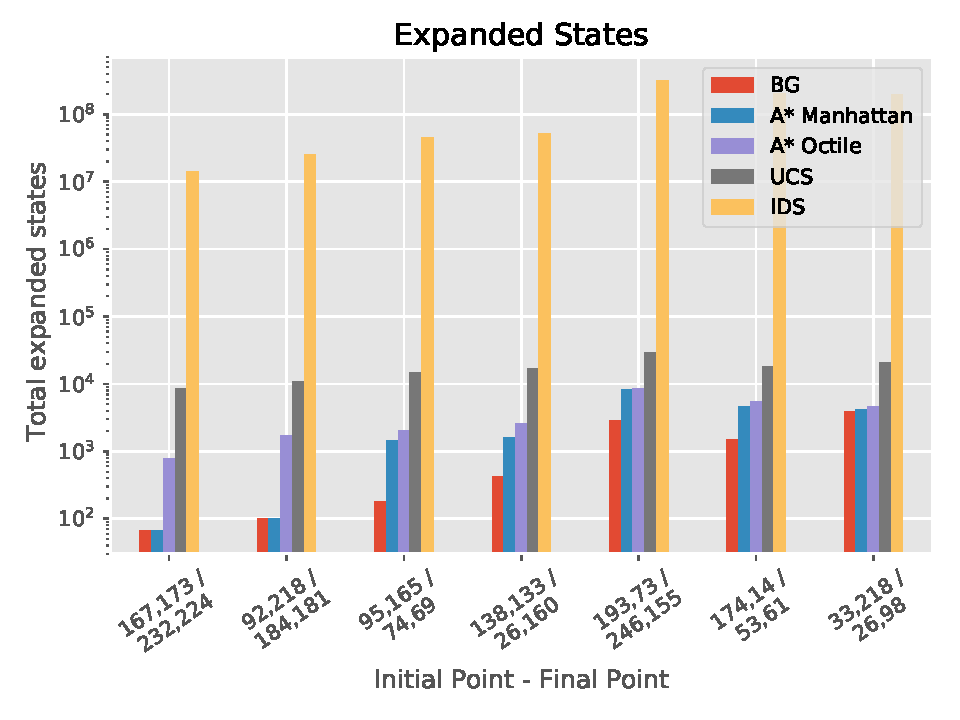
\includegraphics[width=\textwidth]{Images/Expanded_States_map1_log.pdf}
\caption{Estados expandidos para o mapa 1 em escala logarítmica}
\label{fig:expanded1}
\end{minipage}%
\begin{minipage}{0.5\linewidth}
\centering
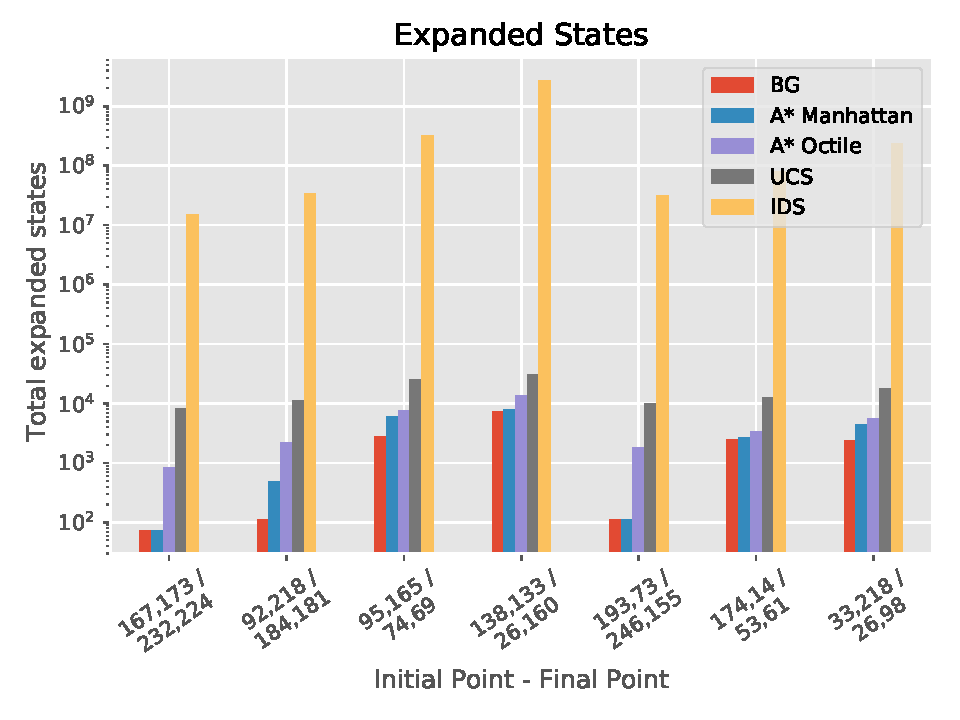
\includegraphics[width=\textwidth]{Images/Expanded_States_map2_log.pdf}
\caption{Estados expandidos para o mapa 2 em escala logarítmica}
\label{fig:expanded2}
\end{minipage}
\begin{minipage}{0.5\linewidth}
\centering
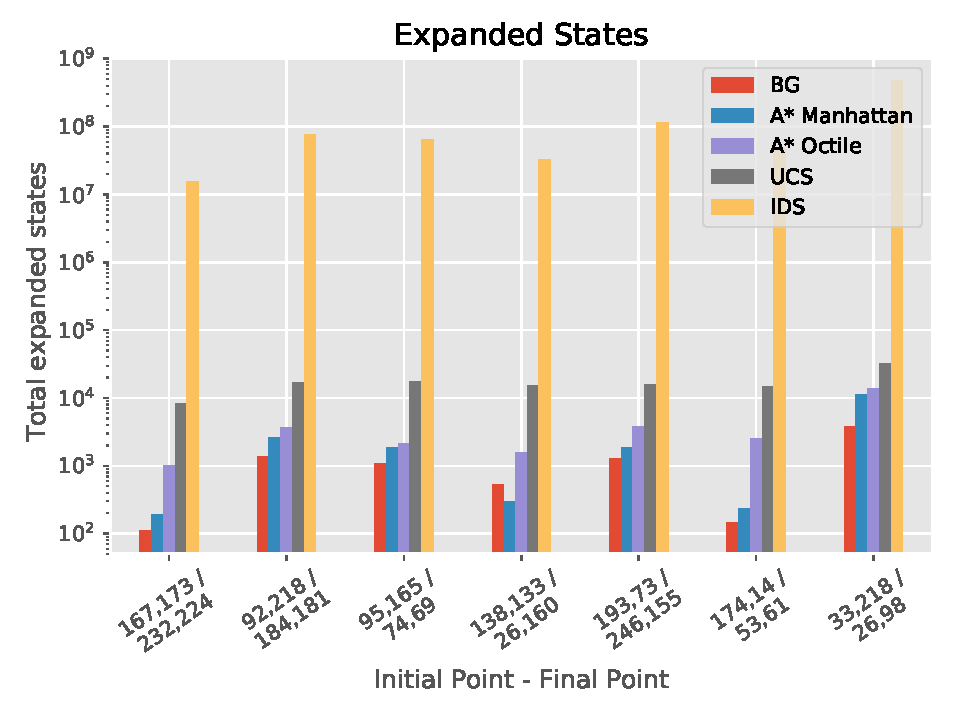
\includegraphics[width=\textwidth]{Images/Expanded_States_map3_log.pdf}
\caption{Estados expandidos para o mapa 3 em escala logarítmica}
\label{fig:expanded3}
\end{minipage}
\end{figure}

O algoritmo de \textit{Best first Search} expande o menor número de estados, devido à sua caraterística gulosa. Isso faz com que o algoritmo muitas vezes não expanda os estados pertencentes à solução ótima. O UCS, expande um número grande de estados comparado com os algoritmos A*, por não ser uma busca com informação. Dessa forma ele precisa buscar muito mais estados pelo objetivo, enquanto o A* possui um certo direcionamento.

\begin{figure}[!htb]
\begin{minipage}{0.5\linewidth}
\centering
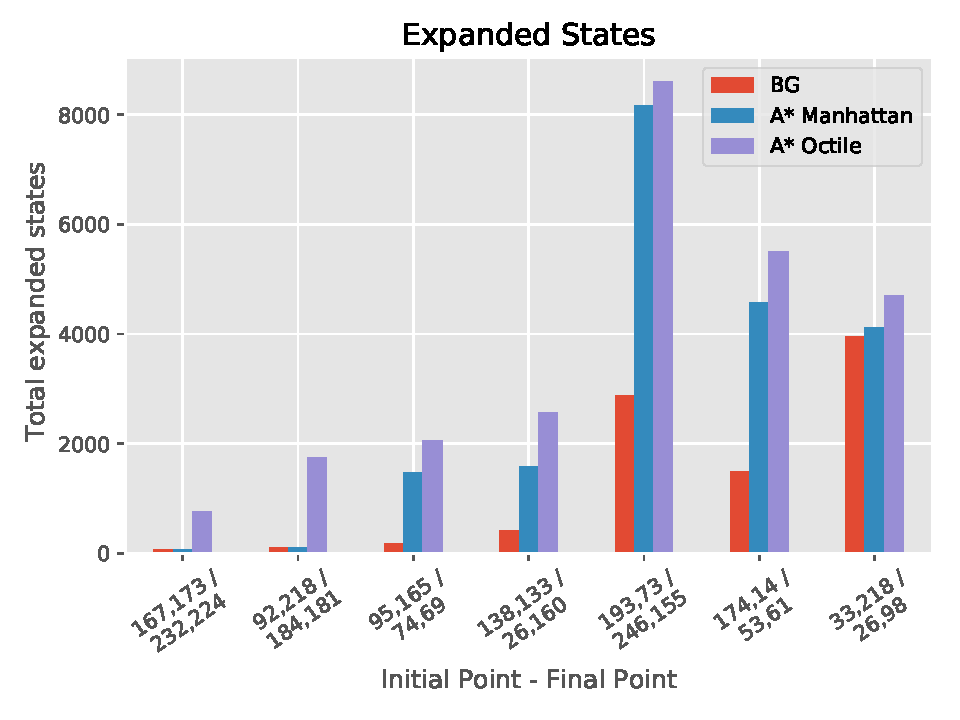
\includegraphics[width=\textwidth]{Images/Expanded_States_map1_log_heuristic.pdf}
\caption{Estados expandidos para as buscas informadas no mapa 1}
\label{fig:expanded-a1}
\end{minipage}%
\begin{minipage}{0.5\linewidth}
\centering
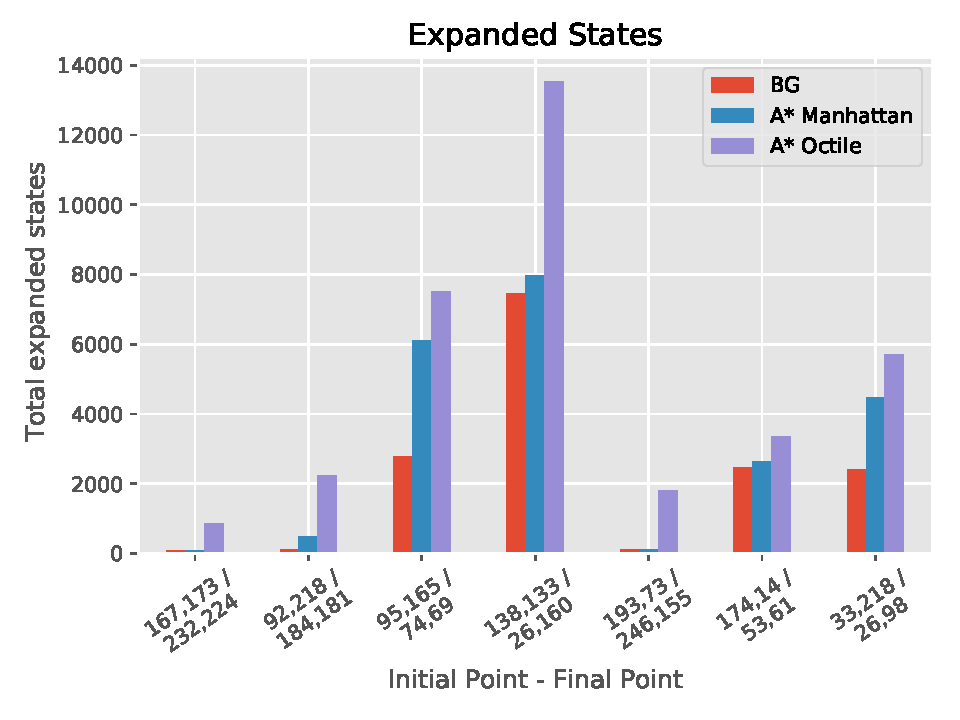
\includegraphics[width=\textwidth]{Images/Expanded_States_map2_log_heuristic.pdf}
\caption{Estados expandidos para as buscas informadas no mapa 2}
\label{fig:expanded-a2}
\end{minipage}
\begin{minipage}{0.5\linewidth}
\centering
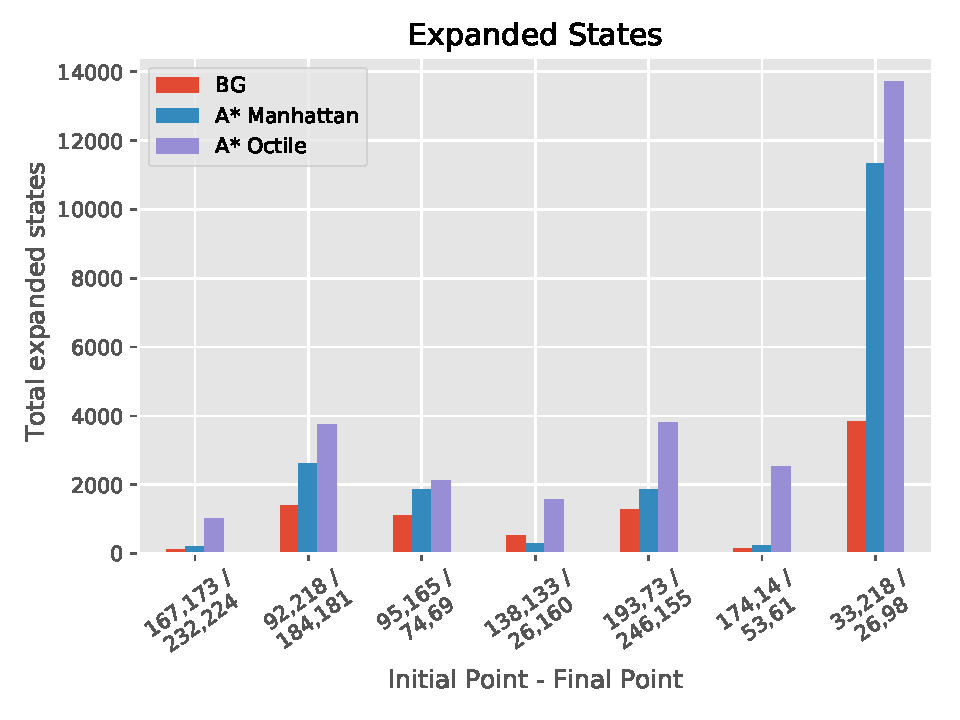
\includegraphics[width=\textwidth]{Images/Expanded_States_map3_log_heuristic.pdf}
\caption{Estados expandidos para as buscas informadas no mapa 3}
\label{fig:expanded-a3}
\end{minipage}
\end{figure}

O número de estados expandidos pelo A* com \textit{distância Manhattan} é menor do que o A* com \textit{distância octile}, como pode ser visto nas figuras~\ref{fig:expanded-a1},~\ref{fig:expanded-a2} e~\ref{fig:expanded-a3}. Dessa forma, o A* com \textit{distância Manhattan} pode não expandir estados que fazem parte do caminho ótimo. Isso é mais uma comprovação de que essa heurística não é admissível e consistente, uma vez que uma heurística consistente expande todos os estados cujo custo é menor do que o ótimo.

O número de estados expandidos por segundo é mostrado nas figuras~\ref{fig:expanded-sec1},~\ref{fig:expanded-sec2} e~\ref{fig:expanded-sec3}. É possível observar que o número de estados expandidos por segundo costuma ser maior para os algoritmos A* em relação ao UCS, em particular nos mapas 1 e 3. Isso ocorre pois esses algoritmos são mais rápidos para encontrar o resultado, expandindo os nós em um período de tempo relativamente menor. O algoritmo de UCS precisa lidar com um número maior de elementos na fronteira conforme ele expande, uma vez os nós são expandidos uniformemente em todas as direções, enquanto o A* expande de uma forma mais direcionada. Para o mapa 2, o número de nós expandidos por segundo para o UCS se mostrou maior em relação ao A* na maioria dos casos. Isso pode ter ocorrido devido a natureza do mapa, que fez com houvesse um número menor de estados para se expandir de uma vez devido a existência de caminhos mais estreitos.

\begin{figure}[!htbp]
\begin{minipage}{0.5\linewidth}
\centering
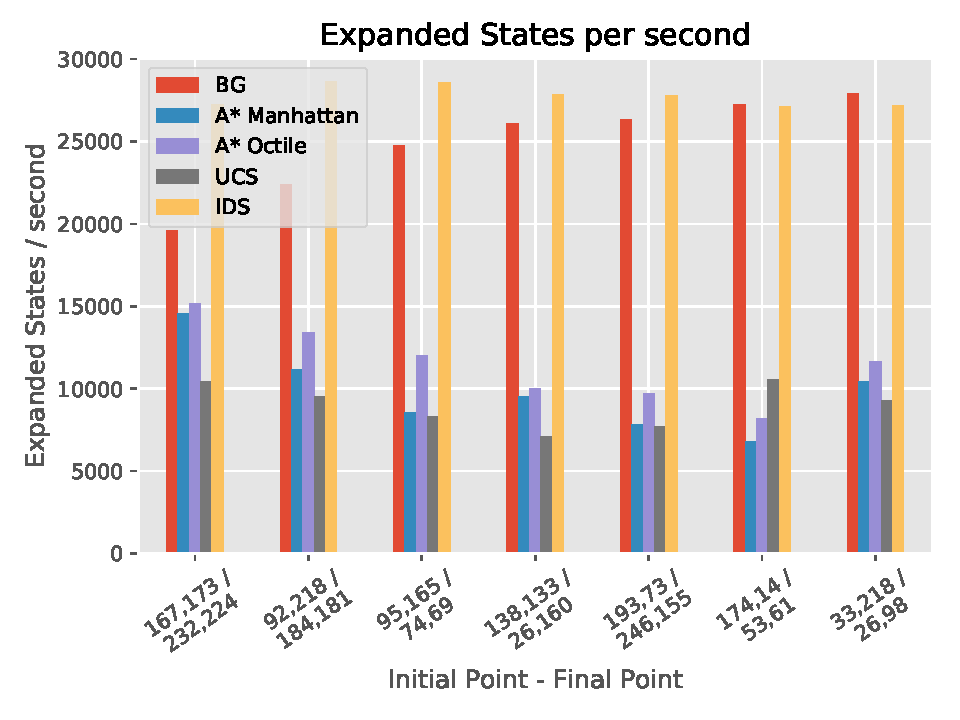
\includegraphics[width=\textwidth]{Images/Expanded_States_sec_map1.pdf}
\caption{Estados expandidos por segundo para o mapa 1}
\label{fig:expanded-sec1}
\end{minipage}%
\begin{minipage}{0.5\linewidth}
\centering
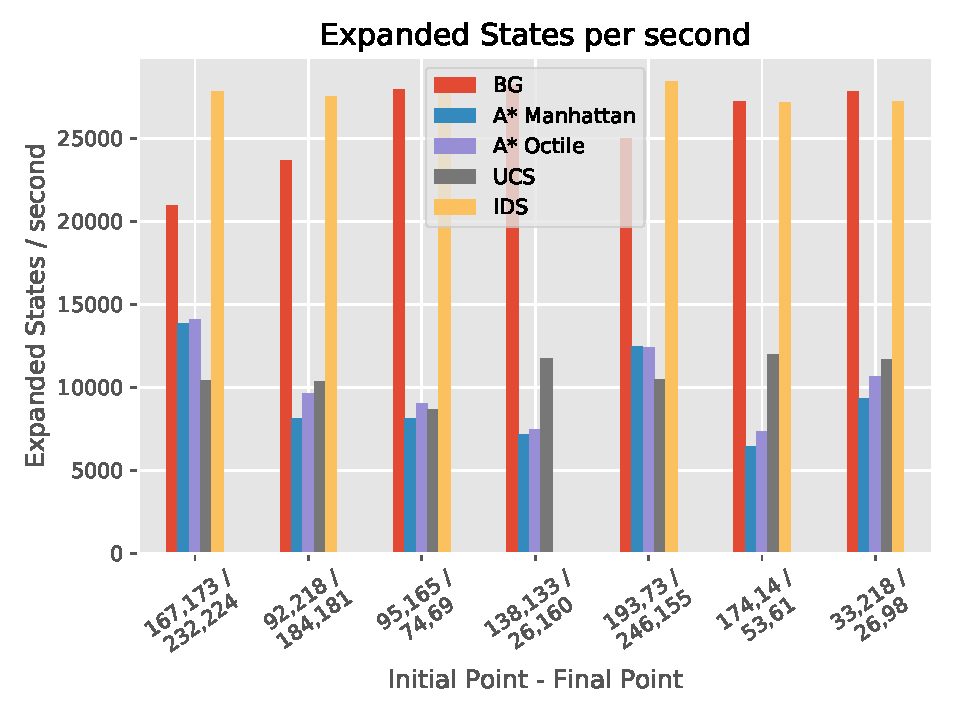
\includegraphics[width=\textwidth]{Images/Expanded_States_sec_map2.pdf}
\caption{Estados expandidos por segundo para o mapa 2}
\label{fig:expanded-sec2}
\end{minipage}
\begin{minipage}{0.5\linewidth}
\centering
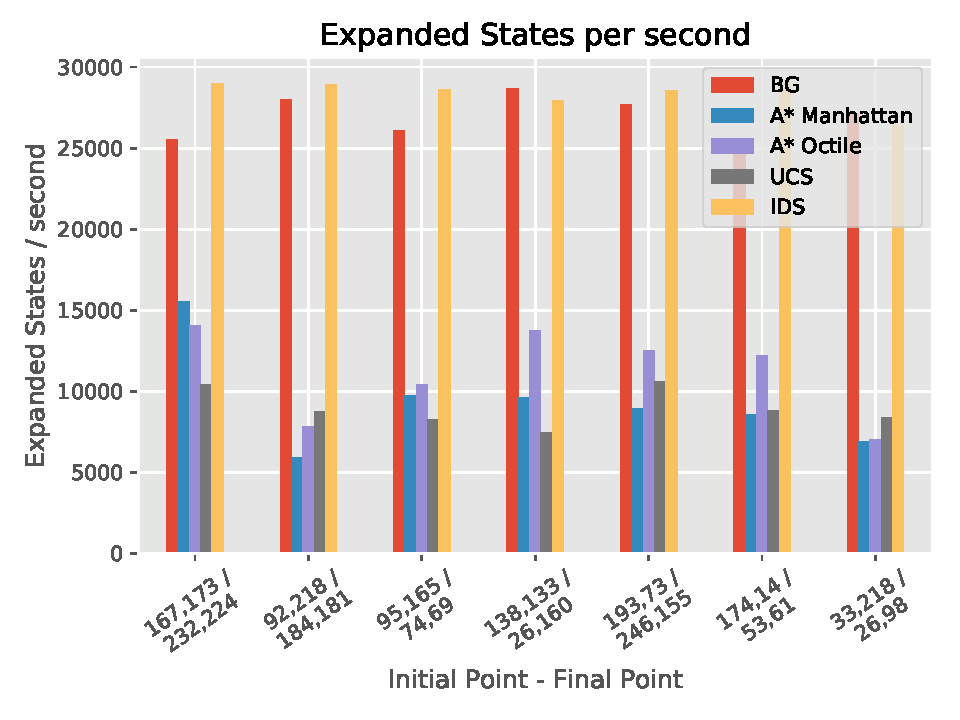
\includegraphics[width=\textwidth]{Images/Expanded_States_sec_map3.pdf}
\caption{Estados expandidos por segundo para o mapa 3}
\label{fig:expanded-sec3}
\end{minipage}
\end{figure}

\subsection{Tempo de execução}

É possível observar que o algoritmo \textit{Best first Search} é o algoritmo mais rápido dentre os examinados. Isso acontece pois ele é um algoritmo guloso, e expande o menor número de estados. O A* é o segundo mais rápido, sendo consideravelmente mais rápido que o UCS. A diferença entre essas três velocidades pode ser vista claramente nas imagens~\ref{fig:time1},~\ref{fig:time2} e~\ref{fig:time3}. O tempo do UCS, o mais lento entre os três, ainda é muito mais rápido do que o tempo do algoritmo IDS. Essas velocidades são um reflexo do número de estados expandidos por cada algoritmo.

\begin{figure}[!htbp]
\begin{minipage}{0.5\linewidth}
\centering
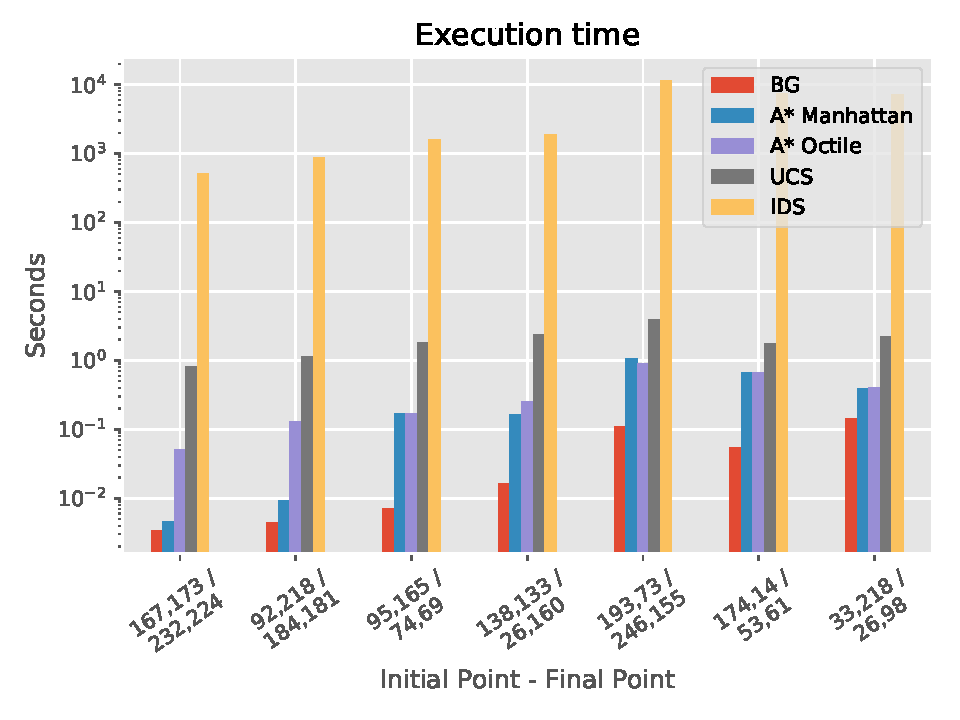
\includegraphics[width=\textwidth]{Images/Execution_time_map1_log.pdf}
\caption{Tempo de execução para o mapa 1 em escala logarítmica}
\label{fig:time1}
\end{minipage}%
\begin{minipage}{0.5\linewidth}
\centering
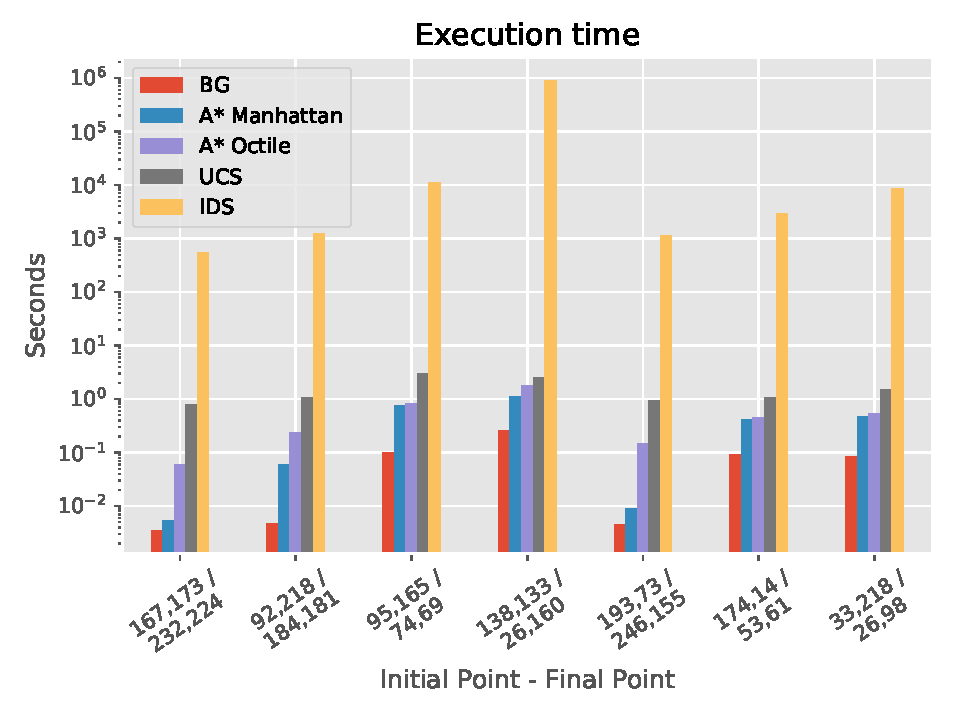
\includegraphics[width=\textwidth]{Images/Execution_time_map2_log.pdf}
\caption{Tempo de execução para o mapa 2 em escala logarítmica}
\label{fig:time2}
\end{minipage}
\begin{minipage}{0.5\linewidth}
\centering
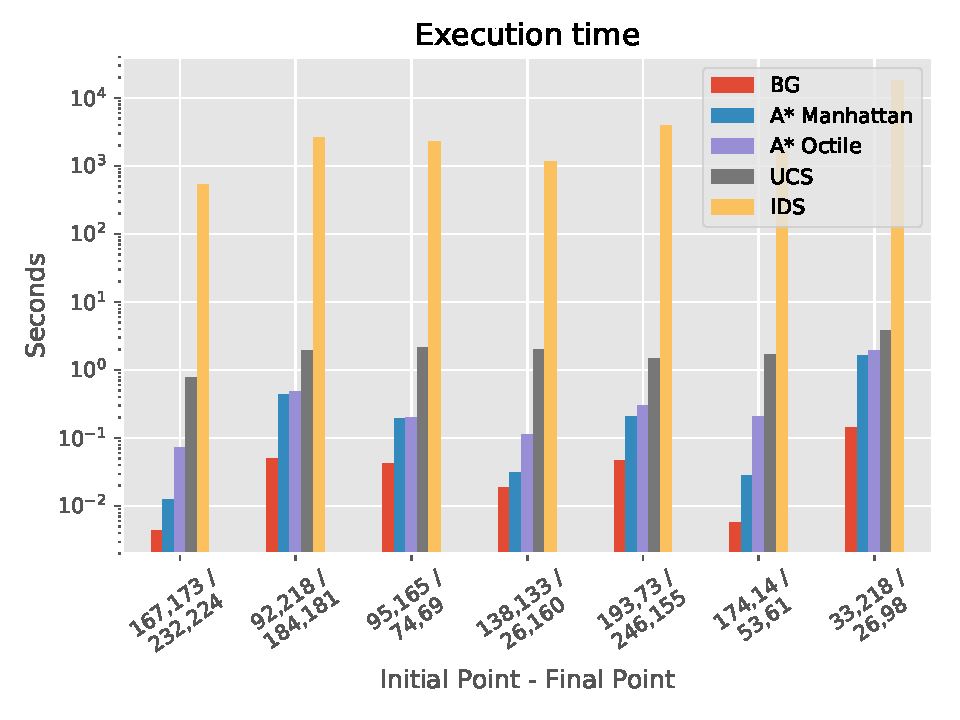
\includegraphics[width=\textwidth]{Images/Execution_time_map3_log.pdf}
\caption{Tempo de execução para o mapa 3 em escala logarítmica}
\label{fig:time3}
\end{minipage}
\end{figure}

Uma comparação melhor entre o tempo de execução dos algoritmos de busca com informação pode ser feita nas imagens~\ref{fig:time1-heur},~\ref{fig:time2-heur} e~\ref{fig:time3-heur}. O algoritmo guloso se mostra mais rápido que o A* em quase todos os exemplos testados. Isso é esperado, devido a sua característica gulosa que faz com que ele busque a primeira solução possível. O A* utilizando \textit{distância Manhattan} é mais rápido do que utilizando \textit{distância octile} na maioria das vezes, uma vez que normalmente expande menos estados.


\begin{figure}[!htb]
\begin{minipage}{0.5\linewidth}
\centering
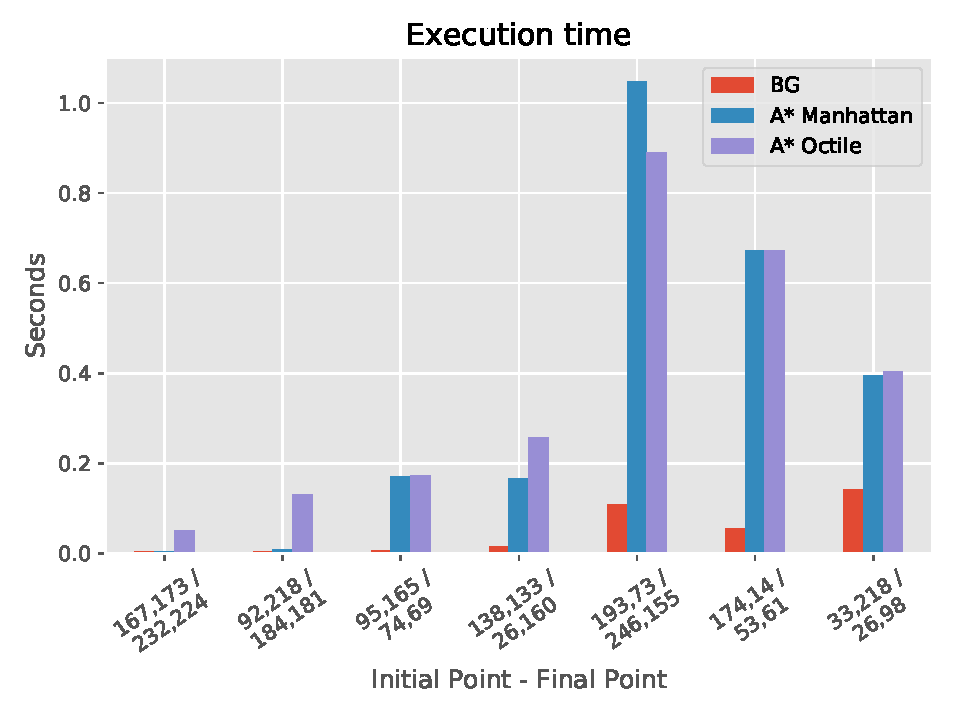
\includegraphics[width=\textwidth]{Images/Execution_time_map1_log_heuristic.pdf}
\caption{Tempo de execução para as buscas informadas no mapa 1 em escala logarítmica}
\label{fig:time1-heur}
\end{minipage}%
\begin{minipage}{0.5\linewidth}
\centering
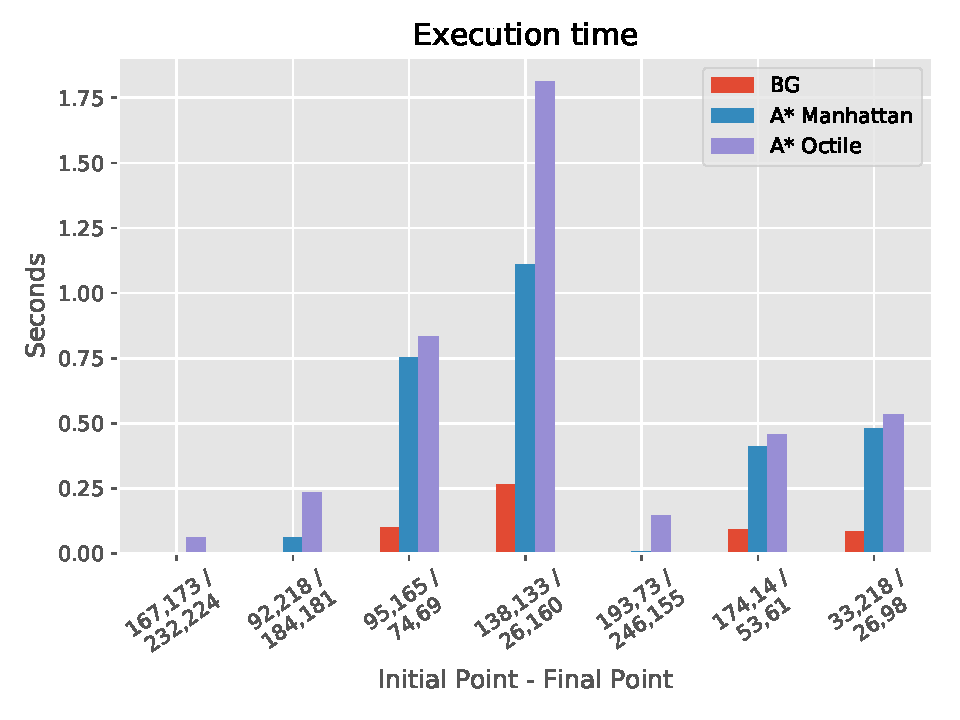
\includegraphics[width=\textwidth]{Images/Execution_time_map2_log_heuristic.pdf}
\caption{Tempo de execução para as buscas informadas no mapa 2 em escala logarítmica}
\label{fig:time2-heur}
\end{minipage}
\begin{minipage}{0.5\linewidth}
\centering
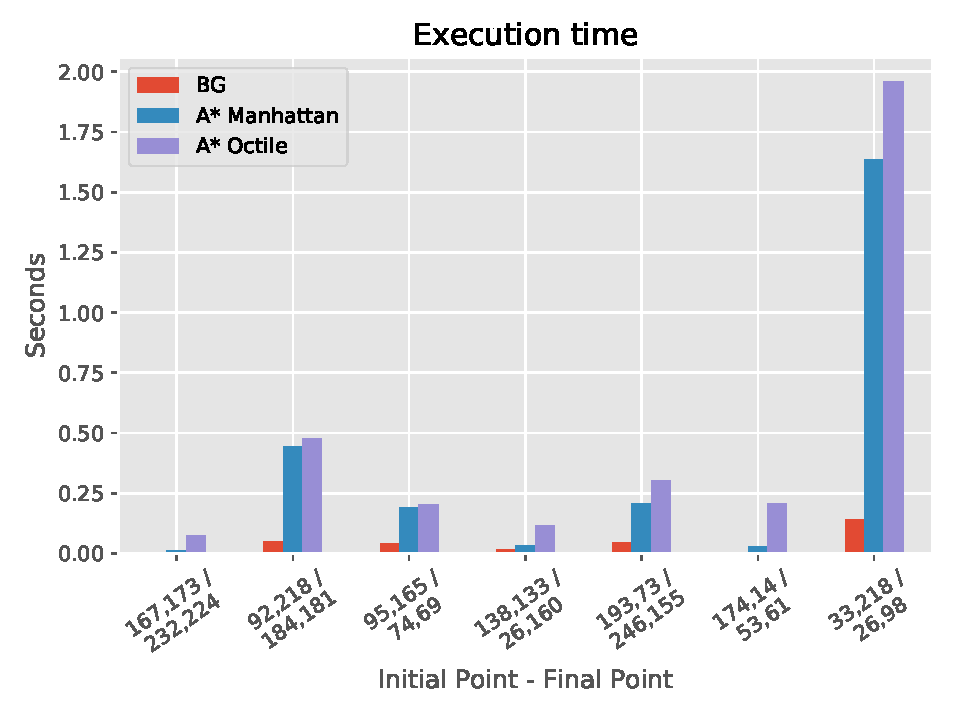
\includegraphics[width=\textwidth]{Images/Execution_time_map3_log_heuristic.pdf}
\caption{Tempo de execução para as buscas informadas no mapa 3 em escala logarítmica}
\label{fig:time3-heur}
\end{minipage}
\end{figure}


\section{Conclusão}
Entre os algoritmos analisados, foi possível perceber claramente uma superioridade entre os algoritmos de busca com informação nos aspectos de tempo e estados expandidos. Isso demonstra a clara vantagem de se possuir algum tipo de conhecimento sobre o espaço em que se está fazendo a busca. Também foi possível observar como a otimalidade do algoritmo A* depende da heurística utilizada. Com uma heurística apropriada, o A* se mostra o algoritmo superior.

Os algoritmos de busca sem informação tiveram um desempenho pior em número de estados expandidos e tempo de execução. O UCS se manteve relativamente próximo ao desempenho dos outros algoritmos, porém o desempenho do algoritmo IDS foi drasticamente inferior até mesmo ao UCS. Seu tempo de execução tornou inviável o teste para distâncias muito grandes. A complexidade de tempo de um DFS normal é $O(b^m)$, onde $m$ é o tamanho máximo de um caminho, o que comparado a complexidade do UCS, $O(b^d)$, onde $d$ é a profundidade da solução mais rasa, é pior. O IDS ainda deve executar um número de iterações igual à profundidade da solução, ou no caso da implementação nesse trabalho, ao custo da solução. Essas diversas iterações tornam o IDS ainda mais lento. Sua vantagem está somente na melhor complexidade de espaço.


\section{Bibliografia}
\bibliographystyle{sbc}
\bibliography{sbc-template}

\end{document}
